\documentclass[noauthor,nooutcomes,12pt]{ximera}

\graphicspath{  
{./}
{./whoAreYou/}
{./drawingWithTheTurtle/}
{./bisectionMethod/}
{./circles/}
{./anglesAndRightTriangles/}
{./lawOfSines/}
{./lawOfCosines/}
{./plotter/}
{./staircases/}
{./pitch/}
{./qualityControl/}
{./symmetry/}
{./nGonBlock/}
}


%% page layout
\usepackage[cm,headings]{fullpage}
\raggedright
\setlength\headheight{13.6pt}


%% fonts
\usepackage{euler}

\usepackage{FiraMono}
\renewcommand\familydefault{\ttdefault} 
\usepackage[defaultmathsizes]{mathastext}
\usepackage[htt]{hyphenat}

\usepackage[T1]{fontenc}
\usepackage[scaled=1]{FiraSans}

%\usepackage{wedn}
\usepackage{pbsi} %% Answer font


\usepackage{cancel} %% strike through in pitch/pitch.tex


%% \usepackage{ulem} %% 
%% \renewcommand{\ULthickness}{2pt}% changes underline thickness

\tikzset{>=stealth}

\usepackage{adjustbox}

\setcounter{titlenumber}{-1}

%% journal style
\makeatletter
\newcommand\journalstyle{%
  \def\activitystyle{activity-chapter}
  \def\maketitle{%
    \addtocounter{titlenumber}{1}%
                {\flushleft\small\sffamily\bfseries\@pretitle\par\vspace{-1.5em}}%
                {\flushleft\LARGE\sffamily\bfseries\thetitlenumber\hspace{1em}\@title \par }%
                {\vskip .6em\noindent\textit\theabstract\setcounter{question}{0}\setcounter{sectiontitlenumber}{0}}%
                    \par\vspace{2em}
                    \phantomsection\addcontentsline{toc}{section}{\thetitlenumber\hspace{1em}\textbf{\@title}}%
                     }}
\makeatother



%% thm like environments
\let\question\relax
\let\endquestion\relax

\newtheoremstyle{QuestionStyle}{\topsep}{\topsep}%%% space between body and thm
		{}                      %%% Thm body font
		{}                              %%% Indent amount (empty = no indent)
		{\bfseries}            %%% Thm head font
		{)}                              %%% Punctuation after thm head
		{ }                           %%% Space after thm head
		{\thmnumber{#2}\thmnote{ \bfseries(#3)}}%%% Thm head spec
\theoremstyle{QuestionStyle}
\newtheorem{question}{}



\let\freeResponse\relax
\let\endfreeResponse\relax

%% \newtheoremstyle{ResponseStyle}{\topsep}{\topsep}%%% space between body and thm
%% 		{\wedn\bfseries}                      %%% Thm body font
%% 		{}                              %%% Indent amount (empty = no indent)
%% 		{\wedn\bfseries}            %%% Thm head font
%% 		{}                              %%% Punctuation after thm head
%% 		{3ex}                           %%% Space after thm head
%% 		{\underline{\underline{\thmname{#1}}}}%%% Thm head spec
%% \theoremstyle{ResponseStyle}

\usepackage[tikz]{mdframed}
\mdfdefinestyle{ResponseStyle}{leftmargin=1cm,linecolor=black,roundcorner=5pt,
, font=\bsifamily,}%font=\wedn\bfseries\upshape,}


\ifhandout
\NewEnviron{freeResponse}{}
\else
%\newtheorem{freeResponse}{Response:}
\newenvironment{freeResponse}{\begin{mdframed}[style=ResponseStyle]}{\end{mdframed}}
\fi



%% attempting to automate outcomes.

%% \newwrite\outcomefile
%%   \immediate\openout\outcomefile=\jobname.oc
%% \renewcommand{\outcome}[1]{\edef\theoutcomes{\theoutcomes #1~}%
%% \immediate\write\outcomefile{\unexpanded{\outcome}{#1}}}

%% \newcommand{\outcomelist}{\begin{itemize}\theoutcomes\end{itemize}}

%% \NewEnviron{listOutcomes}{\small\sffamily
%% After answering the following questions, students should be able to:
%% \begin{itemize}
%% \BODY
%% \end{itemize}
%% }
\usepackage[tikz]{mdframed}
\mdfdefinestyle{OutcomeStyle}{leftmargin=2cm,rightmargin=2cm,linecolor=black,roundcorner=5pt,
, font=\small\sffamily,}%font=\wedn\bfseries\upshape,}
\newenvironment{listOutcomes}{\begin{mdframed}[style=OutcomeStyle]After answering the following questions, students should be able to:\begin{itemize}}{\end{itemize}\end{mdframed}}



%% my commands

\newcommand{\snap}{{\bfseries\itshape\textsf{Snap!}}}
\newcommand{\flavor}{\link[\snap]{https://snap.berkeley.edu/}}
\newcommand{\mooculus}{\textsf{\textbf{MOOC}\textnormal{\textsf{ULUS}}}}


\usepackage{tkz-euclide}
\tikzstyle geometryDiagrams=[rounded corners=.5pt,ultra thick,color=black]
\colorlet{penColor}{black} % Color of a curve in a plot



\ifhandout\newcommand{\mynewpage}{\newpage}\else\newcommand{\mynewpage}{}\fi

\usepackage{fullpage}
\makeatletter
%% no number for activity
\newcommand\logostyle{%
  \def\activitystyle{activity-chapter}
  \def\maketitle{%
                {\flushleft\small\sffamily\bfseries\@pretitle\par\vspace{-1.5em}}%
                {\flushleft\LARGE\sffamily\bfseries\@title \par }%
                {\vskip .6em\noindent\textit\theabstract\setcounter{problem}{0}\setcounter{sectiontitlenumber}{0}}%
                    \par\vspace{2em}
                    \phantomsection\addcontentsline{toc}{section}{\textbf{\@title}}%
                     \setcounter{titlenumber}{0}}}
\makeatother
\newcommand{\nameblankgen}{\noindent\textbf{Name(s) (please print):}\ \hrulefill \\

\hrulefill}
\logostyle



\title[Challenge:]{Design on a plane}
\author{Bart Snapp}

\begin{document}
\begin{abstract}
  We make our own wallpaper patterns.
\end{abstract}
\maketitle

\nameblankgen

\begin{multicols*}{2}

Congratulations! The \mooculus\ Symmetry Squad is impressed by you
preliminary work on frieze patterns. They have a new job for you (again
for points, not cash). Remember how there are $7$ groups of symmetries
for the frieze patters? Well there are $17$ groups of symmetries of
wallpaper patterns. Let's talk about these symmetries.
  

If you have a repeating wallpaper pattern, most folks will agree
it must have at least \emph{two} translational symmetries that are in
\emph{different} directions. Check out my \LOGO:
\begin{logo}
to wallpaper.tt repeat 6 [
pu setxy -240 350-100*repcount seth 90 pd 
repeat 6 [ minimal.cell.t pu fd 100 pd ] ]
end
\end{logo}
Here \lc{minimal.cell.t} is also from our previous work. If you run \lc{wallpaper.tt}, this
produces:
\begin{logoout}
  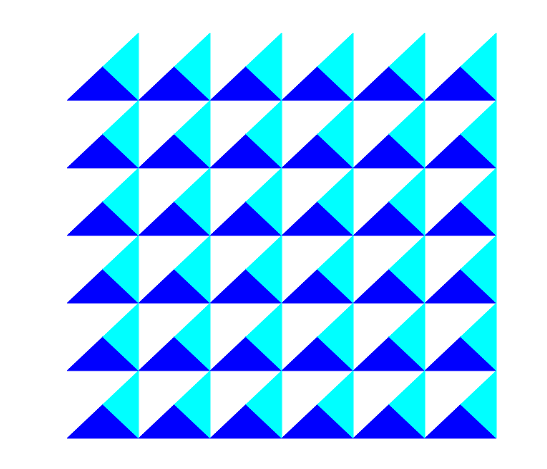
\includegraphics[width=.4\textwidth]{wallpapertt.png}
\end{logoout}
The pattern above has symmetry through a vertical translation and a
horizontal translation, hence \emph{two} translations in
\emph{different} directions. There are also other translations, but
those can be thought of as combos of our vertical and horizontal
translations.  Note these two patterns:
\[
\raisebox{-.5\height}{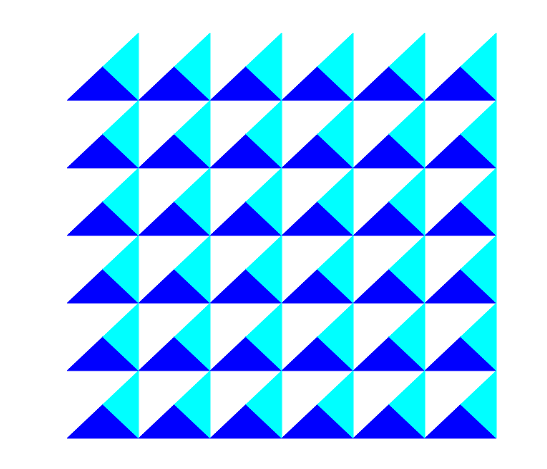
\includegraphics[width=.2\textwidth]{wallpapertt.png}}\quad \text{and} \quad\raisebox{-.5\height}{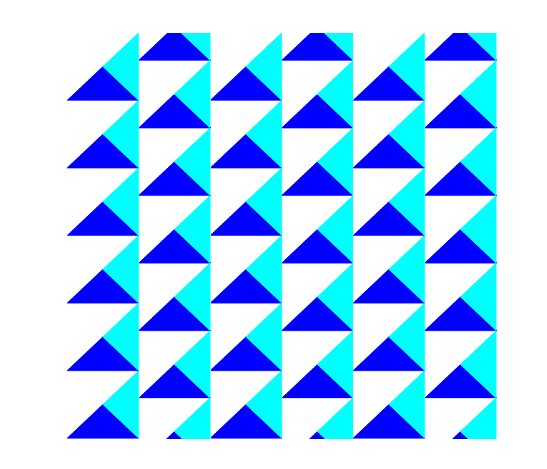
\includegraphics[width=.2\textwidth]{wallpapertt2.png}}
\]
have the \emph{same} symmetry group, though \emph{two translations}.

As a gesture of friendship, I present you with one more wallpaper
pattern with a different group of symmetries:
\begin{logo}
to wallpaper.ttg repeat 6 [
pu setxy -240 350-100*repcount seth 90 pd 
repeat 3 [
  minimal.cell.g pu fd 100 pd ] ]
end
\end{logo}
\begin{logoout}
    \includegraphics[width=.4\textwidth]{wallpaperttg.png}
\end{logoout}
\enlargethispage{\baselineskip}
\end{multicols*}
\newpage


\begin{problem}
  Use \lc{basic.cell :f} to make programs \lc{minimal.cell.X} and
  \lc{wallpaper.Y}, to produce one wallpaper pattern for each possible
  wallpaper symmetry. There are $15$ additional symmetry groups of
  wallpaper patterns. In each case:
  \begin{enumerate}
  \item Display your code. 
  \item Display the output.
  \item List the symmetries of the given wallpaper pattern.
  \end{enumerate}
  As a gesture of friendship, the possible symmetries are: two
  translations (every wallpaper pattern will have these), one/two
  glide reflections, one/two reflectional symmetry, one/two rotational symmetries.
  
\end{problem}

\end{document}
